\begin{abstract}
Soft Tournament Equilibrium (STE) is a differentiable layer for Top-Cycle (TC) and Uncovered-Set (UC) inference from reciprocal pair probabilities. Normalized log-sum-exp reachability and covering give smooth scores with approximation, perturbation, and margin-recovery bounds. We distinguish structural supervision, posterior uncertainty, and the final set decision through controlled synthetic studies and reconstruction of recorded ordinal profiles. Matched-epoch training improves F1 under a common structural readout, but a separate equal-budget soft-UC comparison does not demonstrate an advantage. A prospective equal-budget hard-UC study improves selective F1 at 24 alternatives from 0.6327/0.6292 for ordinary/relational native heads to 0.6676, while exact recovery remains only 1.16\%. On 36 human profiles held out by source, a separate exploratory comparison favors Jeffreys posterior inference over learned independent-edge and mixture distributions in native expected-F1 decoding (0.8742 versus 0.8704/0.8366). Only three references are non-singleton selective cores. Completion certificates and full-depth TC diagnostics clarify additional identification, smoothing, and computational limits. The evidence supports conditional synthetic overlap gains, while preserving the soft-set null and the absence of a demonstrated learning advantage over strong count-based human-profile controls.
\end{abstract}

\section{Introduction}\label{sec:intro}
Pairwise comparisons support preference learning and model evaluation, but their majority relation can cycle: $a$ defeats $b$, $b$ defeats $c$, and $c$ defeats $a$. Heterogeneous contexts can produce cycles even when each context is ordered. Language-model evaluations exhibit non-transitivity \citep{xu2025nontransitivity}; other work ensembles evaluators or filters toward acyclic relations \citep{hu2026acyclic,yu2025elspr}. A ranking and a mutually competitive leading set answer different questions.

Classical tournament solutions provide structural targets \citep{brandt2016handbook,laslier1997tournament}. The \emph{Top Cycle} (TC) consists of alternatives that can reach every other alternative along majority-win paths. The \emph{Uncovered Set} (UC) excludes an alternative when another defeats it and every opponent it defeats. Both select the Condorcet winner when one exists. Unlike a fixed-size ranking shortlist, these sets are determined by the relation itself. Their hard definitions, however, are discontinuous in estimated edge probabilities near a majority tie.

\emph{Soft Tournament Equilibrium} (STE) maps pair probabilities to continuous TC/UC scores. Equilibrium denotes a tournament core rather than a Nash equilibrium or fixed point. Smoothing reachability and covering lets core labels supervise the pair predictor. We ask when differentiating through a tournament solution helps: relation learning, soft selection, and deployed decisions need not improve together. A separate posterior branch describes model-based membership uncertainty.

\begin{figure*}[t]
\centering
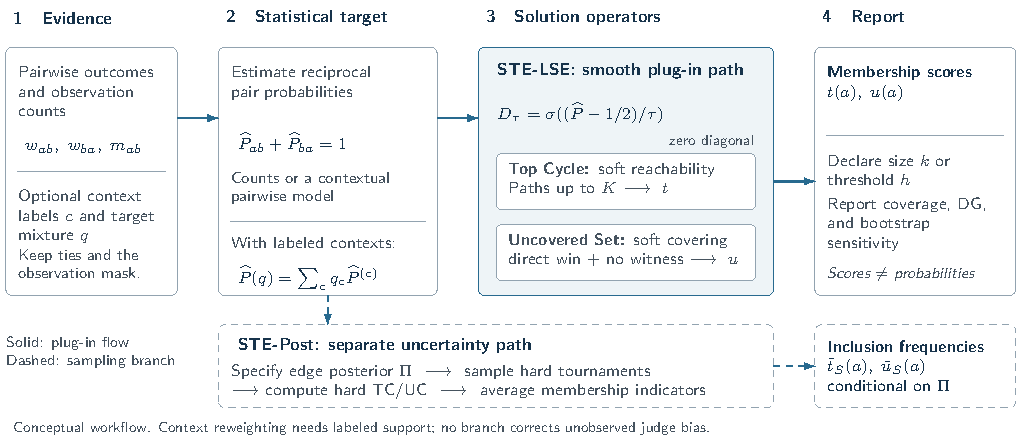
\includegraphics[width=0.92\textwidth]{figures/fig_ste_overview_v4.pdf}
\caption{\textbf{STE inference workflow.} Comparison records define reciprocal pair probabilities. STE-LSE computes smooth TC/UC scores for supervision; STE-Post averages hard memberships under a specified posterior. Reporting a set requires a separate decision rule. Training differentiates the smooth scores, not the selected set.}
\label{fig:overview}
\end{figure*}

We contribute smooth TC/UC operators, approximation and perturbation bounds, and counterexamples separating scores from posterior and hard membership. Three twelve-collection GPU studies compare structural supervision under matched epochs and equal budgets. Whole-source human-profile studies evaluate the complete decision against count-only and fitted posterior controls, including a learned dependent orientation model. Completion-based certificates separate logically justified membership from unresolved edges. Recorded-core reconstruction and gradient/cost diagnostics retain their separate scopes; oracle size is diagnostic only.

\noindent\textbf{Relation to prior work.} TC and UC are established social-choice objects \citep{good1971note,smith1973aggregation,miller1980graph,fishburn1977condorcet}. Fuzzy spatial-voting models study covering and uncovered sets under indifference \citep{mordeson2011uncovered}; STE instead smooths majority and core predicates into differentiable membership scores for supervision. Bradley--Terry--Luce (BTL), Rank Centrality, and HodgeRank fit scalar or spectral rankings \citep{bradley1952rank,luce1959individual,negahban2017rank,jiang2011statistical}. UCB-style dueling-bandit algorithms identify TC, UC, and other winning sets through active comparisons \citep{ramamohan2016dueling}; STE takes a supplied probability matrix. Differentiable sorting relaxes an ordering \citep{blondel2020fast}, and generic perturbed optimizers smooth discrete solution maps \citep{berthet2020learning}. Soft Condorcet Optimization learns scalar ratings for a ranking objective \citep{lanctot2024sco}; STE differentiates core membership of a potentially cyclic relation. Margin-of-victory methods measure edge changes needed to alter membership \citep{brill2022margin}. Our contribution is the explicit smooth TC/UC construction, its error analysis, and its controlled evaluation as a training layer.



\section{Statistical target and hard cores}\label{sec:problem}
Let $\agents=\{1,\ldots,n\}$, $n\ge2$, and let $P_{ab}$ be the probability that $a$ defeats $b$ under a declared evaluation distribution. We use \emph{reciprocal} probabilities, $P_{ab}+P_{ba}=1$ and $P_{aa}=1/2$; the corresponding margins or logits, not $P$ itself, are antisymmetric. Counts $w_{ab}$ and $w_{ba}$ summarize $m_{ab}=w_{ab}+w_{ba}$ decisive comparisons. Our primary estimand conditions on a decisive outcome. Observed ties are recorded separately rather than treated as wins.

\noindent\textbf{The comparison distribution is part of the target.} For labeled contexts, write $P^{(c)}_{ab}=\Pr(a\succ b\mid a,b,c,\text{decisive})$ and define $P(q)=\sum_c q_cP^{(c)}$ with declared pair-independent weights. These standardize context-conditional decisive relations. Discarding ties from pooled observations generally induces different weights when tie rates vary by pair/context; observing pairs on different tasks also need not identify this mixture. Reweighting requires labels, support, and a stated target distribution (Appendix~\ref{app:decisive-mixtures}).

For $P_{ab}\ne1/2$ on every unordered pair, $T(P)$ is the strict tournament with edge $a\to b$ iff $P_{ab}>1/2$. Exact ties are allowed in $P$, but omitting both directions produces an incomplete directed graph, not a strict tournament.
\begin{figure}[t]
\centering
% Deterministic example: all six strict-majority edges, no fitted data.
% Circles mark UC members; the square marks the covered vertex. All are in TC.
\begin{tikzpicture}[
  >=Stealth,
  every node/.style={font=\fontsize{7.2}{8.4}\selectfont},
  ucvertex/.style={circle,draw=steBlue,line width=.65pt,fill=steBlue!7,
    minimum size=4.9mm,inner sep=0pt},
  coveredvertex/.style={rectangle,draw=steGray,line width=.65pt,fill=steGray!13,
    minimum size=4.9mm,inner sep=0pt},
  majority/.style={-{Stealth[length=2.0mm,width=1.35mm]},draw=steGray,line width=.55pt},
  certificate/.style={-{Stealth[length=2.0mm,width=1.35mm]},draw=steBlue,line width=.75pt},
  panel/.style={anchor=north west,align=left,inner sep=0pt,text width=5.25cm}
]
% Bounding box: about one column wide and 3.0 cm high.
\path[use as bounding box] (-.22,-.60) rectangle (7.83,2.40);
\node[anchor=west,inner sep=0pt,font=\fontsize{7.2}{8.4}\selectfont\bfseries]
  at (-.06,2.20) {(a) Tournament};
\node[ucvertex] (a) at (0,1.74) {$a$};
\node[ucvertex] (b) at (1.95,1.74) {$b$};
\node[ucvertex] (c) at (.975,.12) {$c$};
\node[coveredvertex] (d) at (.975,.95) {$d$};

% Arrowless annotation drawn first: majority edges remain visually continuous.
\draw[draw=steGray,densely dashed,line width=.35pt]
  (d.east) -- (2.36,.95) |- (2.53,.43);

% Exactly six majority edges. Blue edges certify that b covers d.
\draw[majority] (a) -- (b);
\draw[majority] (c) to[bend left=15] (a);
\draw[certificate,preaction={draw=white,line width=2.3pt}]
  (b) to[bend left=16] (c);
\draw[majority] (a) -- (d);
\draw[certificate] (b) -- (d);
\draw[majority] (d) -- (c);

\node[anchor=west,inner sep=0pt,font=\fontsize{7.2}{8.4}\selectfont\bfseries]
  at (2.53,2.20) {(b) Membership certificates};
\node[panel] at (2.53,1.93) {
  $N^+(a)=\{b,d\},\quad N^+(b)=\{c,d\}$\\[2pt]
  $N^+(c)=\{a\},\qquad N^+(d)=\{c\}$
};
\node[panel] at (2.53,1.15) {
  \textbf{TC:} $\{a,b,c,d\}$ (full panel)\\[2pt]
  $d\to c\to a\to b\to d$ is a spanning cycle.
};
\node[panel,fill=white] at (2.53,.51) {
  \textbf{UC:} $b$ covers $d$ $\Rightarrow\UC=\{a,b,c\}$\\[2pt]
  $b\to d,\quad N^+(d)=\{c\}\subset N^+(b)$
};

% Explicit shape and line semantics make the figure readable in monochrome.
\node[ucvertex,minimum size=2.4mm] at (.02,-.39) {};
\node[anchor=west,inner sep=0pt,font=\fontsize{6.7}{7.4}\selectfont]
  at (.21,-.39) {UC member};
\node[coveredvertex,minimum size=2.4mm] at (2.03,-.39) {};
\node[anchor=west,inner sep=0pt,font=\fontsize{6.7}{7.4}\selectfont]
  at (2.22,-.39) {covered};
\node[anchor=west,inner sep=0pt,font=\fontsize{6.7}{7.4}\selectfont]
  at (3.62,-.39) {All nodes: TC};
\node[anchor=west,inner sep=0pt,font=\fontsize{6.7}{7.4}\selectfont,text=steBlue]
  at (5.65,-.39) {Blue: cover proof};
\end{tikzpicture}

\caption{One relation, distinct TC and UC targets. Solid arrows show all six majority edges; blue edges certify that $b$ covers $d$. Circles mark UC members and the square marks covered $d$. The spanning cycle certifies full TC. The dashed leader is an annotation, not an edge.}
\label{fig:worked-tournament}
\end{figure}
\Needspace{8\baselineskip}
\begin{definition}[TC and UC on a strict tournament]\label{def:cores}
With self-reachability understood, $\TC(T)=\{a:a\leadsto_T b\ \forall b\in\agents\}$. For distinct $c,a$, $c$ \emph{covers} $a$ iff $c\to a$ and $a\to b$ implies $c\to b$ for every $b\notin\{a,c\}$. Then $\UC(T)=\{a:\nexists c\text{ covering }a\}$.
\end{definition}
Reachability and covering can also be evaluated on incomplete graphs, without inheriting strict-tournament properties. We identify this convention when observed pairs are missing or tied. Figure~\ref{fig:worked-tournament} shows a strict tournament with distinct cores.

\noindent\textbf{What missing comparisons leave unidentified.} Observing only $a\to b$ and $b\to c$ permits two completions: $a\to c$ gives $\TC=\UC=\{a\}$, while $c\to a$ gives $\{a,b,c\}$. Neutral imputation does not distinguish them. We retain the observation mask and distinguish soft estimation from certified hard membership.

\section{Soft tournament inference}\label{sec:method}
\subsection{Edge estimation and canonical operators}
The edge estimator is modular. An unrestricted differentiable scorer $g_\theta$ can give
\begin{equation}\label{eq:learner}
\begin{split}
h_\theta(a,b,x)&=g_\theta(a,b,x)-g_\theta(b,a,x),\\
P_\theta(a\succ b\mid x)&=\sigma(h_\theta(a,b,x)),
\end{split}
\end{equation}
where $\sigma(z)=(1+e^{-z})^{-1}$ and $x$ is a comparison context. Pairwise cross-entropy can fit this model. A scalar scorer $s_\theta(a,x)$ gives the restricted contextual BTL logit $s_\theta(a,x)-s_\theta(b,x)$. This enforces transitivity within a context, not necessarily after marginalizing contexts. Our count experiments use $\widehat P_{ab}=(w_{ab}+1/2)/(m_{ab}+1)$, including $\widehat P_{ab}=1/2$ for missing pairs.

For edge temperature $\tau>0$, define
\begin{equation}\label{eq:edge}
D_\tau(a,b)=\begin{cases}0,&a=b,\\ \sigma((P_{ab}-1/2)/\tau),&a\ne b.\end{cases}
\end{equation}
For a nonempty $r$-vector $z$, normalized log-sum-exp (LSE) extrema are
\begin{equation}\label{eq:extrema}
\begin{split}
\smax_\gamma(z)&=\gamma\log\!\left(r^{-1}\sum_{i=1}^r e^{z_i/\gamma}\right),\\
\smin_\gamma(z)&=-\smax_\gamma(-z).
\end{split}
\end{equation}
They map $[0,1]^r$ into $[0,1]$ and approximate max/min within $\gamma\log r$. Normalization preserves the score range but makes finite-temperature values sensitive to aggregation size; it is not probability calibration. Temperatures $\tau,\gamma,\gamma_c$ respectively smooth majority edges, paths, and covering; they do not estimate observation noise. Tying them is an experimental choice.

\subsection{Top-Cycle membership}
Hard reachability is an OR over paths of an AND over their edges. Define the smooth max--min product
\begin{equation}\label{eq:product}
(X\otimes_\gamma Y)_{ab}=\smax_\gamma\{\smin_\gamma(X_{ac},Y_{cb}):c\in\agents\}.
\end{equation}
With $Q^{(1)}=D_\tau$ and $Q^{(k)}=Q^{(k-1)}\otimes_\gamma D_\tau$, set
\begin{align}
R(a,b)&=\smax_\gamma\{Q^{(k)}(a,b):1\le k\le K\},\label{eq:reach}\\
t(a)&=\smin_\gamma\{R(a,b):b\ne a\}.\label{eq:tc}
\end{align}
In the hard limit, the inner minimum tests a path's weakest edge, the maximum tests existence of a path, and the final minimum requires reachability to every opponent. Full TC recovery requires $K\ge n-1$; a smaller $K$ is a bounded-depth surrogate. At positive temperature the nested operations are a particular smooth recurrence, not a probability that a path exists: overlapping walks reuse edges, and normalized soft extrema are not Boolean probabilities.

\subsection{Uncovered-Set membership}
A counterexample to ``$c$ covers $a$'' is an opponent beaten by $a$ but not by $c$. Its soft score is
\begin{equation}\label{eq:violation}
v(c,a)=\smax_{\gamma_c}\{D_\tau(a,b)(1-D_\tau(c,b)):b\notin\{a,c\}\}.
\end{equation}
Use $v(c,a)=0$ for an empty witness set ($n=2$), and define
\begin{align}
\operatorname{cov}(c,a)&=D_\tau(c,a)(1-v(c,a)),\quad c\ne a,\\
u(a)&=1-\smax_{\gamma_c}\{\operatorname{cov}(c,a):c\ne a\}.\label{eq:uc}
\end{align}
UC does not use $R$ or $K$. Its witness test is local to triples $(c,a,b)$, whereas TC aggregates paths through the whole graph. The two scores answer different structural questions and need not select the same finite-temperature shortlist. 

\begin{algorithm}[t]
\caption{Canonical STE-LSE forward pass}\label{alg:lse}
\small
\noindent\textbf{Input:} $P\in[0,1]^{n\times n}$, $P_{ab}+P_{ba}=1$, $P_{aa}=1/2$; $n\ge2$, $\tau,\gamma,\gamma_c>0$, integer $K\ge1$.
\par\smallskip
\begingroup
\setlength{\tabcolsep}{0pt}
\renewcommand{\arraystretch}{1.02}
\begin{tabular}{@{}r@{\hspace{0.55em}}p{\dimexpr\linewidth-2em\relax}@{}}
1 & Set $D_{aa}\gets0$; for $a\ne b$, set $D_{ab}\gets\sigma((P_{ab}-1/2)/\tau)$.\\
2 & $Q\gets D$, $L\gets D/\gamma$.\\
3 & \textbf{for} $k=2,\ldots,K$:\\
4 & \quad Allocate a new $n\times n$ matrix $Q^{\rm new}$.\\
5 & \quad\textbf{for} $b\in\agents$, write column $b$ of $Q^{\rm new}$:\\
6 & \qquad $H_{ac}\gets\smin_\gamma(Q_{ac},D_{cb})$ for all $a,c$.\\
7 & \qquad $Q^{\rm new}_{ab}\gets\smax_\gamma\{H_{ac}:c\in\agents\}$ for all $a$.\\
8 & \quad $Q\gets Q^{\rm new}$; $L\gets\operatorname{logaddexp}(L,Q/\gamma)$.\\
9 & $R\gets\gamma(L-\log K)$, entrywise.\\
10 & $t_a\gets\smin_\gamma\{R_{ab}:b\ne a\}$ for all $a$.\\
11 & \textbf{for} $a\in\agents$:\\
12 & \quad\textbf{for} $c\in\agents\setminus\{a\}$:\\
13 & \qquad If $n=2$, set $v(c,a)\gets0$; otherwise set\\
14 & \qquad $v(c,a)\gets\smax_{\gamma_c}\{D_{ab}(1-D_{cb}):b\notin\{a,c\}\}$.\\
15 & \qquad $\operatorname{cov}(c,a)\gets D_{ca}(1-v(c,a))$.\\
16 & \quad $u_a\gets1-\smax_{\gamma_c}\{\operatorname{cov}(c,a):c\ne a\}$.\\
17 & \textbf{return} continuous scores $t,u$, before any set decision.\\
\end{tabular}
\endgroup
\end{algorithm}


\subsection{Variants and uncertainty}\label{sec:variants}
Eqs.~\eqref{eq:edge}--\eqref{eq:uc} define \LSE; Algorithm~\ref{alg:lse} gives a streamed forward reference, separate from the GPU implementation (Appendix~\ref{app:ibm-gpu}). The historical \WB\ variant instead confidence-weights edges, uses Boltzmann UC aggregation, and exact max--min TC paths. Its equations and 64,800-instance archive are distinguished in Appendix~\ref{app:variant-details}; the GPU studies use \LSE.

\textbf{STE-Post} instead samples a hard tournament from a specified edge posterior and averages hard memberships. For example, independent edge posteriors derived from symmetric Beta priors produce $\bar u_S(a)=S^{-1}\sum_s\mathbf1\{a\in\UC(T^{(s)})\}$. These frequencies describe the chosen posterior, not a model-free probability of membership. None of these procedures estimates judge quality or corrects unobserved judge bias.  

\subsection{Selection and core-supervised learning}\label{sec:training-objective}
A score vector $z$ becomes a reported set only after specifying a rule, such as $S_h(z)=\{a:z_a\ge h\}$. We select $h$ on separate development tournaments and hold it fixed on tests. This selects a decision rule, not calibrated probabilities or an oracle size. The distinction between smooth scores, posterior inclusion, and hard membership is formalized in Section~\ref{sec:score-meaning}.

For a minibatch of observed graphs $W$ and associated labels $y_a=\mathbf1\{a\in C(T)\}$, $C\in\{\TC,\UC\}$, we use
\begin{equation}\label{eq:coretraining}
\mathcal L(\theta)=\mathcal L_{\rm pair}(P_\theta;W)
+\lambda\operatorname{BCE}(f_C(P_\theta),y).
\end{equation}
Here $f_{\TC}=t$, $f_{\UC}=u$, and $\mathcal L_{\rm pair}$ normalizes by the total comparison count in the minibatch; BCE averages across its graphs and alternatives. Gradients pass through soft reachability or covering and the reciprocal pair predictor, not through $S_h$. Section~\ref{sec:learning} compares this objective with pairwise-only training and a direct membership head using the same target-specific core labels. Synthetic experiments use latent-generator cores; exploratory human-profile learning uses full-record empirical cores from training sources. These references do not supply population truth.

\section{Error bounds and context transfer}\label{sec:theory}
We separate approximation, estimation, and changes in the target. Appendix~\ref{app:proofs} provides complete proofs and recovery certificates. These supplied-matrix guarantees establish neither optimization convergence nor predictor generalization.

\begin{theorem}[Finite-temperature core approximation]\label{thm:finite}
Let $M$ be a strict tournament adjacency, $D\in[0,1]^{n\times n}$ have zero diagonal, $\eta=\|D-M\|_\infty$, and $K\ge n-1$. The canonical STE-LSE scores satisfy
\begin{align}
\|t(D)-\mathbf1_{\TC(M)}\|_\infty
&\le\eta+\gamma\{(K-1)\log n+\log K\},\label{eq:tc-bound}\\
\|u(D)-\mathbf1_{\UC(M)}\|_\infty
&\le3\eta+\gamma_c\log(n-1).\label{eq:uc-bound}
\end{align}
Each bound may be capped at one. If it is below $\min(h,1-h)$, thresholding at $h\in(0,1)$ recovers the hard set; $h=1/2$ maximizes this allowance.
\end{theorem}
The proof tracks the under-approximation from normalized soft maxima separately from the over-approximation from soft minima, avoiding the sum of opposing smoothing allowances. For strict-margin $P$ with $\Delta=\min_{a\ne b}|P_{ab}-1/2|>0$ and $\|\widehat P-P\|_\infty\le\epsilon<\Delta$, Eq.~\eqref{eq:edge} gives $\eta\le e^{-(\Delta-\epsilon)/\tau}$. At fixed finite $n,K$, uniform consistency and temperatures tending to zero yield hard-core consistency and Condorcet inclusion. Exact ties do not identify a unique strict orientation.

The bounds are sufficient, not necessary. Even the sharpened TC smoothing term exceeds $1/2$ at $n=12$, $K=11$, $\gamma=0.035$, and exceeds one at $n=24$; it grows with $K\log n$. It therefore does not certify the GPU study's operating points. Binary target structure sharpens UC's edge term to $2\eta-\eta^2$ (Appendix~\ref{rem:uc-binary-refinement}), without changing the operator. More observations reduce statistical error, but neither fixed smoothing bias nor posterior Monte Carlo precision. Missing pairs still require identification assumptions.

Let $t_0$ use ordinary maxima/minima in the same TC recurrence. Under Theorem~\ref{thm:finite}'s assumptions, Appendix~\ref{app:tc-certificates} proves
\[
|t_a(D)-\mathbf1_{\TC(M)}(a)|
\le\min\{1,\eta+|t_a(D)-t_{0,a}(D)|\}.
\]
The computable smoothing discrepancy still needs a valid uniform edge-error allowance $\eta$; average pair MSE does not suffice. A separate one-sided refinement uses members' shortest-path lengths. Both preserve the operator without certifying unchecked recorded operating points.

\begin{proposition}[Fixed-temperature perturbations]\label{prop:lipschitz}
For reciprocal $P,P'$ of the same size, fixed positive temperatures, and the same $K\ge1$, let $e=\|P-P'\|_\infty$. STE-LSE satisfies
\begin{equation}\label{eq:regularity}
\begin{split}
\|t(P)-t(P')\|_\infty&\le e/(4\tau),\\
\|u(P)-u(P')\|_\infty&\le 3e/(4\tau).
\end{split}
\end{equation}
These inequalities do not require strict majority margins.
\end{proposition}
Hard memberships can jump when an edge crosses $1/2$; Eq.~\eqref{eq:regularity} bounds smooth-score perturbations even there. Smaller $\tau$ sharpens the hard approximation but increases worst-case sensitivity to probability error. The TC perturbation constant is independent of $K$, whereas its \emph{approximation bias} in Theorem~\ref{thm:finite} accumulates with depth.

\begin{proposition}[Nonuniform comparison counts]\label{prop:sample}
Suppose each unordered pair has $m_{ab}>0$ independent Bernoulli observations with mean $P_{ab}$ and margin $\Delta_{ab}=|P_{ab}-1/2|>0$. For the raw empirical mean $\widehat P$,
\begin{equation}\label{eq:sample}
\Pr\{T(\widehat P)\ne T(P)\}\le 2\sum_{a<b}e^{-2m_{ab}\Delta_{ab}^2}.
\end{equation}
On the complementary event, both hard cores agree. Independence across different pairs is not needed for this union bound.
\end{proposition}
For uniform $m$ and minimum margin $\Delta$, this reduces to $n(n-1)e^{-2m\Delta^2}$. Corollary~\ref{cor:finite-sample-recovery} combines this concentration argument with edge smoothing and Theorem~\ref{thm:finite} to certify thresholded scores under the stated Bernoulli model. Missing pairs and pseudocount bias require separate treatment.

\begin{proposition}[Mixture transfer with weight error]\label{prop:mixture}
Let context probabilities $P^{(c)}$ be unchanged between training and evaluation, with $\|\widehat P^{(c)}-P^{(c)}\|_\infty\le\epsilon_c$. For target weights $q$ and estimated weights $\widehat q$ in the probability simplex,
\begin{equation}\label{eq:mixture}
\left\|\sum_c\widehat q_c\widehat P^{(c)}-\sum_cq_cP^{(c)}\right\|_\infty
\le \sum_c\widehat q_c\epsilon_c+\tfrac12\|\widehat q-q\|_1.
\end{equation}
If this bound is below the target's strict majority margin, both induced hard cores agree.
\end{proposition}
Known weights eliminate the last term; context support and stable conditional probabilities remain essential. Appendix~\ref{app:proofs} also bounds model-conditional posterior Monte Carlo error.


% Optional main-text insertion. The defining result and complete proof are in
% sections/posterior_certificates_theory.tex; do not duplicate theorem numbering.
\paragraph{Posterior decisions and logical certificates.}
A tournament law and a rule for reporting its UC are separate objects. GFM uses the joint moments $\Pr(i\in\UC(T),|\UC(T)|=s\mid D)$ to maximize modeled expected F1 \citep{waegeman2014fmeasure}; membership marginals alone omit its size-dependent denominator. Shared mixture components also induce dependent edges, so multiplying mixture edge marginals generally gives a different law.

Known orientations can alternatively bound UC without recovering every edge. Define $I(G)$ as vertices with known paths of length at most two to every opponent, and exclude $v$ from $O(G)$ when a known $u\to v$ has, for each $w\notin\{u,v\}$, known $w\to v$ or $u\to w$. Proposition~\ref{prop:uc-completion-enclosure} proves $I(G)\subseteq\UC(T)\subseteq O(G)$ for every strict completion $T$; equality certifies the complete set. This applies established two-step tournament supports \citep{aziz2015partial,contet2026supports}. Fixed-design i.i.d. pair intervals make the enclosure simultaneous with probability $1-\delta$ (Corollary~\ref{cor:uc-fixed-design-enclosure}). That sampling claim does not apply to finite human-cohort subsampling, and the certificate establishes no adaptive-query or comparison-budget savings. Appendix~\ref{app:posterior-certificates-theory} gives complete proofs and the separate mixture-training identity.


\subsection{What a soft UC score means}\label{sec:score-meaning}
A bounded smooth score is neither a calibrated membership probability nor a certificate of correct ordering. The following constructions separate these interpretations; their full proofs are in Appendix~\ref{app:proofs}.

\begin{lemma}[Neutral-input UC reference]\label{lem:neutral}
For $n\ge3$, if $P_{ab}=1/2$ for all distinct $a,b$, then the canonical UC score is $u_a=5/8$ for every alternative and every positive $\tau,\gamma_c$.
\end{lemma}
Equal neutral witness scores give $v=1/4$ and cover strength $3/8$, regardless of temperature. Thus an unobserved graph under neutral imputation can score above one half without directional evidence.

\begin{lemma}[Distinct plug-in and posterior summaries]\label{lem:distinct-summaries}
Let $\Pi$ be uniform on the eight strict three-vertex tournaments, encoded by $0/1$ edge probabilities and diagonal $1/2$. At every positive canonical temperature, $u_a(\mathbb E_\Pi P)=5/8$ but $\Pr_\Pi\{a\in\UC(T(P))\}=1/2$ for each vertex.
\end{lemma}
Six transitive tournaments and two cycles give four UC inclusions per vertex. Plug-in and posterior summaries are intrinsically different.

\begin{proposition}[A finite-temperature ordering counterexample]\label{prop:ordering-counterexample}
There is a reciprocal strict-margin probability matrix with known entries whose hard TC and UC are the singleton $\{a\}$, but whose canonical UC scores at $\tau=\gamma_c=0.035$ satisfy $u(b)>u(a)$. Consequently no upper-threshold rule or descending-score prefix recovers that singleton at these temperatures.
\end{proposition}
The construction uses $P_{ab}=P_{ac}=0.501$, $P_{bc}=0.9$: exact probabilities do not eliminate smoothing bias.


\section{Experiments}\label{sec:experiments}
The matched-epoch study, equal-budget soft-UC comparison, and prospective hard-UC confirmation retain distinct frozen primary families. Both human-profile learning studies are exploratory; the posterior-control extension uses a previously examined cohort. Appendices~\ref{app:ibm-gpu}--\ref{app:real-learning} and~\ref{app:posterior-native} give protocols, controls, and audits. Historical studies, oracle cardinalities, and latent probabilities remain separate diagnostics.

For a reported set $S$ and reference core $C$, F1 is $2|S\cap C|/(|S|+|C|)$, with value one when both are empty. Exact recovery is $\mathbf1\{S=C\}$; size is $|S|$. We average these per-graph quantities rather than pooling vertex decisions across graphs. Core classes are singleton, selective non-singleton ($1<|C|<n$), and full ($|C|=n$). Both overlap and exact recovery matter: a large selection can achieve useful F1 while failing to identify the core.

\begin{table}[t]\centering\scriptsize
{\setlength{\tabcolsep}{1.2pt}
\begin{tabular*}{\linewidth}{@{\extracolsep{\fill}}lrrrrlrr@{}}
\toprule
Core & $n$ & STE & Aux. & $\Delta$ F1 & 95\% CI & $p_{\rm Holm}$ & Pos.\\
\midrule
UC & 24 & .6078 & .5761 & $+.0317$ & $[.0182,.0453]$ & .0015 & 12/12\\
UC & 48 & .4931 & .4638 & $+.0293$ & $[.0102,.0484]$ & .0127 & 11/12\\
TC & 24 & .5405 & .5111 & $+.0294$ & $[.0109,.0480]$ & .0127 & 10/12\\
\bottomrule
\end{tabular*}
}

\caption{Frozen primary contrasts under the same structural readout and development-selected cutoff. $\Delta$ is STE minus auxiliary F1; CI uses $t_{11}$ over twelve collection means, each averaging graphs and three initializations. Two-sided exhaustive sign-flip tests receive Holm adjustment over these three endpoints. Pos. counts positive collection effects.}
\label{tab:gpu-primary}\end{table}

\subsection{Separate UC and TC structural training}\label{sec:learning}
Twelve independent collections contain 512 training and 128 development graphs at $n=12$, and 256 tests at each $n\in\{12,24,48,64\}$. Three paired initializations share each collection. The 12,288 distinct tests cross ordered, planted cyclic, TC/UC-separated, context-mixture, and random families. Heterogeneous comparison counts, planned missingness 0.25, and tie probability 0.2 produce the observations; latent conditional-decisive majority cores supply labels. Singleton, selective, and full cores are reported separately.

UC and TC train separately with a shared $16\to32\to32$ reciprocal pair encoder taking counts, ties, and masks. Auxiliary and STE objectives receive identical core labels; ordinary and relational heads add active parameters. Candidates receive 160 paired Adam epochs. Development selects loss weight, checkpoint, and readout cutoff. Full TC uses $K=n-1$ with checkpointing; temperatures are 0.035. Equal epochs do not match compute: STE TC/UC steps cost 3.66$\times$/4.10$\times$ auxiliary steps at $n=12$ (Appendix~\ref{app:ibm-gpu}).



The matched-readout gains are 0.0317/0.0293 for UC at $n=24/48$ and 0.0294 for TC at $n=24$ (Table~\ref{tab:gpu-primary}). Auxiliary heads train for their own membership predictions, whereas STE trains through the structural decoder: this comparison measures decoder alignment, not complete-system superiority. Intervals use twelve independent collection effects; exact sign flipping assumes null sign-reversal exchangeability. Graphs and initializations are not additional independent units.

\textbf{Native readouts.} Auxiliary heads have higher TC F1. STE exceeds the relational head by 0.0210/0.0262 UC F1 at $n=24/48$, but both heads are stronger at the training size $n=12$ (Table~\ref{tab:gpu-systems}). These descriptive comparisons use each readout's development selection; active capacities and compute differ.

\textbf{Selective cores and cardinality.} UC matched-readout gains are 0.0376/0.0370 on selective non-singletons at $n=24/48$, versus 0.0087/0.0007 on full cores. TC's $n=24$ gain is concentrated on singletons (0.0693 versus 0.0062 on selective cores). Selective UC exact recovery is only 5.76\%/1.79\%; selections average 13.16/29.34 versus reference sizes 9.66/13.13 (Table~\ref{tab:selective-recovery}). These descriptive strata expose over-inclusion when a cutoff selected at $n=12$ transfers to larger panels.

\subsection{Equal-budget UC complete systems}\label{sec:equal-compute}
The soft-UC follow-up uses twelve fresh collections, three paired initializations, and the unchanged generators/operator. Each system receives 220 synchronized seconds, including training, native-readout development selection, and serialization. Development selective UC F1 selects loss weight, one of five checkpoints, and a cutoff before test generation. Setup/test evaluation are excluded; every candidate and system passes the fixed $\pm2\%$ timing gate (Appendix~\ref{app:uc-equal-compute}).

\begin{table}[t]\centering\scriptsize
\begin{tabular*}{\linewidth}{@{\extracolsep{\fill}}lrr}
\toprule
Objective / readout & $n=24$ & $n=48$ \\
\midrule
Pair / structural & $0.6245\pm0.0043$ & $0.4018\pm0.0061$ \\
Aux. / head & $0.6414\pm0.0085$ & $0.4280\pm0.0068$ \\
Rel. aux. / head & $0.6416\pm0.0061$ & $0.4263\pm0.0051$ \\
STE / structural & $0.6281\pm0.0074$ & $0.4076\pm0.0046$ \\
\bottomrule
\end{tabular*}

\caption{Equal-budget native systems: selective non-singleton UC F1, mean $\pm$ SEM across twelve collections, each averaging three initializations. Only $n=24$ is primary; $n=48$ is descriptive. SEM is not a confidence interval.}
\label{tab:uc-equalcompute-main}\end{table}

At the primary $n=24$ endpoint, STE minus ordinary/relational direct heads is $-0.01329/-0.01345$, with individual 95\% $t_{11}$ intervals $[-0.03286,0.00628]/[-0.03300,0.00611]$. Both exact sign-flip tests have Holm-adjusted $p=0.3193$ in this separate two-test family. The study does not demonstrate an equal-budget advantage; it establishes neither inferiority nor equivalence. The studies differ in compute, readout, and endpoint, precluding attribution to compute alone.

The original checkpoints also yield a post hoc hard-decoding benefit and lower pair MSE (Appendix~\ref{app:uc-equal-compute}). Those descriptive outputs retain their original status and motivated the separate test below.

\subsection{Prospective hard-UC confirmation}\label{sec:hard-confirm}
A fresh frozen protocol compares six separately trained systems with decoder-aligned development selection (Appendix~\ref{app:hard-confirm}). Each receives 220 charged seconds per paired initialization; every candidate and complete system passes the unchanged $\pm2\%$ gate. STE still trains through soft UC, while checkpoint/loss-weight selection and deployment use hard UC of $\widehat P_{ab}>1/2$, without a membership cutoff. Native ordinary/relational heads and separately trained hard-decoded controls receive their own selection.

\begin{table}[t]\centering\scriptsize\setlength{\tabcolsep}{2pt}
\begin{tabular*}{\linewidth}{@{\extracolsep{\fill}}lrrr@{}}\toprule
System / readout & F1, $n=24$ & F1, $n=48$ & \shortstack{Exact (\%)\\$n=24$}\\\midrule
Pair / hard & 0.5865 (0.0078) & 0.4012 (0.0056) & 1.45\\
Ordinary / native & 0.6327 (0.0045) & 0.4309 (0.0042) & 2.02\\
Relational / native & 0.6292 (0.0051) & 0.4318 (0.0055) & 2.53\\
STE / hard & 0.6676 (0.0043) & 0.5159 (0.0030) & 1.16\\
Ordinary / hard & 0.5972 (0.0082) & 0.4121 (0.0060) & 1.41\\
Relational / hard & 0.6237 (0.0031) & 0.4324 (0.0053) & 1.44\\
\bottomrule\end{tabular*}

\caption{Prospective equal-budget UC systems on selective cores. F1 is mean (SEM) over twelve collections, each averaging three initializations; exact recovery is a percentage. Only STE-hard versus native heads at $n=24$ belongs to the separate two-test primary family; other entries are descriptive.}
\label{tab:hard-confirm-main}\end{table}

At primary $n=24$, STE-hard F1 is 0.6676 versus 0.6327/0.6292 for ordinary/relational native heads. Paired differences are 0.03493/0.03843, with individual 95\% $t_{11}$ intervals $[0.02383,0.04602]/[0.02763,0.04922]$; both exhaustive sign-flip tests have Holm-adjusted $p=0.00098$. All twelve collection effects are positive. This supports the tested hard-UC pipeline without replacing the soft-set null. Exact recovery is only 1.16\%, below the heads' 2.02/2.53\%; at $n=48$, selections average 25.99 versus 13.13 reference members. Overlap gains do not establish exact or size-faithful recovery.

\subsection{Count inference and automatic decisions}\label{sec:counts}
Count controls share observations and development calibration without test core size. Posterior inference uses 512 Beta$(1/2,1/2)$ edge-posterior draws; GFM optimizes their expected F1 \citep{waegeman2014fmeasure}. Appendix~\ref{app:ibm-gpu} gives all decision controls.

UC STE-LSE/posterior/Rank Centrality F1 is 0.5459/0.4583/0.5386 at $n=24$ and 0.3930/0.3569/0.4424 at $n=64$. TC at $n=24$ favors count-only Rank Centrality (0.5494) over both count STE (0.4669) and learned STE (0.5405). Rank Centrality uses the same observations and development labels for its cutoff, without supervised model fitting. These descriptive comparisons reuse the learning collections. Latent-$P$ and oracle-size outputs are diagnostic; full baselines and stopping checks are in Appendix~\ref{app:ibm-gpu}.

\subsection{Strict selective recorded-profile reconstruction}\label{sec:profiles}
We reparse 462 original PrefLib ordinal profiles from eleven source series, retaining record multiplicities, tied ranks, and unranked alternatives \citep{mattei2013preflib}. Eligibility is determined from raw observations before method performance. The primary UC cohort requires every decisive pair observed, no exact empirical majority ties, $1<|\UC|<n$, and no exact within-source count duplicate. Twelve profiles from four sources qualify, spanning 4--24 alternatives and 51--28,660 ordinal records. Eleven have UC size three and one has size twelve, limiting cardinality diversity.

\textbf{Source identity matters.} Only three qualifying profiles are human elections: two ERS elections and one Oakland election \citep{preflibers,oneill2013openstv}. The other nine are two Multilaps and seven Formula 1 profiles whose rankings encode athletes' lap times \citep{boehmer2022collecting}. PrefLib's generic ``voters'' field does not imply human judgments. This is a mixed recorded-ranking benchmark, not a twelve-profile human-preference validation (Appendix~\ref{app:gpu-real-inventory}).

The reference is the complete finite-profile empirical core. Ten whole-record resampling streams use nested 10\%, 25\%, and 50\% fractions. Calibration excludes the test source and equally weights the others. The primary setting is UC at 25\% records without extra missingness; repetitions average within profiles, profiles within sources, and the four sources equally. This tests count reconstruction, not neural transfer or population truth (Appendix~\ref{app:ibm-gpu}).

\begin{table}[t]\centering\small
\begin{tabular}{@{}lrr@{}}
\toprule
Method & UC F1 & Exact (\%)\\
\midrule
STE-LSE & 0.6491 & 9.64\\
Posterior core & 0.7824 & 32.32\\
Posterior GFM & 0.6920 & 11.43\\
Smooth Copeland & 0.6820 & 22.50\\
BTL & 0.6561 & 6.43\\
Copeland & 0.6548 & 27.50\\
Rank Centrality & 0.5689 & 5.71\\
Native hard UC & 0.5535 & 11.07\\
Select all & 0.5163 & 0.00\\
Select none & 0.0000 & 0.00\\
\bottomrule
\end{tabular}

\caption{Strict selective recorded UC reconstruction at the frozen 25\%-record setting: three election and nine sports profiles, four equally weighted sources. Score methods use source-excluded absolute calibration; GFM and hard/all/none controls use native decisions. Exact is complete-set recovery.}
\label{tab:gpu-real}\end{table}

Posterior UC has F1 0.7824 versus STE-LSE 0.6491 and exact recovery 32.32\% versus 9.64\% (Table~\ref{tab:gpu-real}). All four source effects favor posterior inference. The descriptive STE-minus-posterior $t_3$ interval is $[-0.3454,0.0788]$; shared calibration sources preclude a source-population coverage guarantee. Secondary TC and partial/tied references remain separate in Appendix~\ref{app:ibm-gpu}.

The edge-factorized posterior is a working model: ordinal records create dependent pairs, laps may be serially dependent, and its latent random core differs from the finite reference. Subsampling measures reconstruction of that record set, not future-race prediction. Three election profiles are insufficient to establish broad human-preference utility.

\textbf{Exploratory human-profile learning.} A separate study fits the pair model on 36 human ordinal profiles from six source series. Each whole-source fold uses four sources for training, one for development, and one for testing (Appendix~\ref{app:real-learning}). References are full-record empirical UC; only three are selective and 33 are singletons. At 10\% sampled records, equal-source macro F1 is 0.8745 for STE soft selection and 0.8808 for STE hard UC, below count-hard 0.9002 and posterior-half 0.9016. STE soft exact recovery is 80.65\% versus 85.03/83.23\% for those controls. These are exploratory finite-record reconstruction results, with no p-values or population/general-superiority claims; the cohort and prior estimator outcomes were already inspected.

\subsection{Native posterior and count controls on human profiles}\label{sec:posterior-native}
A separate extension on the same 36-profile cohort tests learned predictive distributions against strong count-based controls (Appendix~\ref{app:posterior-native}). It preserves the earlier human-profile results. Six whole-source folds hold out one source for testing and one for development; eight nested whole-record subsamples and three paired initializations retain actual rank multiplicities. All methods receive observed decisive/tied counts at test time. Jeffreys and fitted symmetric empirical-Bayes edge posteriors, learned independent orientations, and a learned two-component tournament distribution use native GFM expected-F1 decisions. Ordinary/relational heads use their own development-selected cutoffs; raw-count UC uses its native covering rule. The fitted systems share a 120-second upper allocation, with actual costs reported separately.

\begin{table}[t]\centering\scriptsize\setlength{\tabcolsep}{3pt}
\begin{tabular*}{\linewidth}{@{\extracolsep{\fill}}lrrr@{}}\toprule
System & F1 & Exact & UC Brier\\\midrule
Jeffreys--GFM & \textbf{0.8742} & 0.7656 & 0.0437\\
Empirical Bayes--GFM & 0.8705 & 0.7522 & 0.0447\\
Learned edges--GFM & 0.8704 & 0.7614 & \textbf{0.0400}\\
Learned mixture--GFM & 0.8366 & 0.7301 & 0.0486\\
Raw-count UC & 0.8481 & \textbf{0.7950} & ---\\
Relational head & 0.7944 & 0.6161 & 0.0681\\
Ordinary head & 0.7340 & 0.5730 & 0.0708\\\midrule
Count soft plug-in (secondary) & 0.8462 & 0.7679 & 0.0507\\\bottomrule
\end{tabular*}
\caption{Exploratory native decisions at 10\% records: mean within profile, then source, then six equally weighted sources. Exact is complete-set recovery; lower UC Brier measures agreement of membership scores with the finite reference. The cohort has 33 singleton and three selective targets. No significance or population-calibration claim is made.}
\label{tab:posterior-native-main}\end{table}

Jeffreys--GFM has the highest native F1, and raw-count UC the highest exact recovery (Table~\ref{tab:posterior-native-main}). Learned edges nearly match Jeffreys F1 and have lower recorded UC Brier; the mixture does not improve either endpoint. On the three selective targets, each of size three, Jeffreys F1 is 0.8411 versus 0.6749/0.6542 for learned edges/mixture. Their selections average 2.72 versus 1.70/1.58 members. No native method exactly recovers the eleven-alternative ERS profile in any saved 10\% input. These two-source selective means are descriptive, with no p-values or general superiority claim. An independent raw-output review verifies native decoding and selected-checkpoint replay, and excludes an invalid mixture hard-decoding diagnostic caused by floating-point self-loops (Appendix~\ref{app:posterior-native}).

\subsection{TC fidelity, gradients, and measured cost}\label{sec:gpu-diagnostics}
GPU diagnostics use three graphs per family/size at $n=8,16,32,64,96$, three temperatures, and four depths including $K=n-1$. At the default temperature and full depth, the \emph{long-path family} has mean absolute TC score error rising from 0.218 at $n=8$ to 0.847 at $n=96$; ordered and planted errors remain much smaller (Figure~\ref{fig:gpu-tc-error}). Score error differs from selected-set F1: selecting all can recover a full core.

\begin{figure}[t]\centering
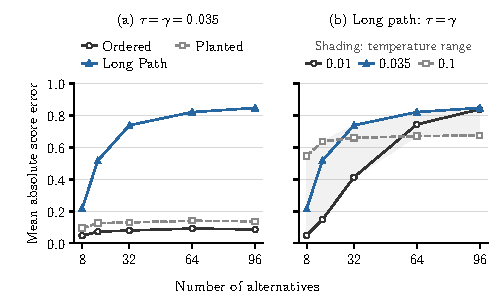
\includegraphics[width=\columnwidth]{figures/v10_tc_error.pdf}
\caption{Full-depth TC score error ($K=n-1$). (a) Families at $\tau=\gamma=0.035$. (b) Long-path sensitivity with $\tau=\gamma$; shading spans means at the three tested temperatures, not a confidence band. Each point averages vertex errors over three saved graphs. These are operator diagnostics, not trained-model transfer tests.}
\label{fig:gpu-tc-error}\end{figure}

Diagnostic gradients differentiate clipped BCE with respect to probability logits. They are finite, but low-temperature cells can have negligible or zero entries; no lower bound on useful training signal follows. All 540 plain/checkpoint pairs have identical outputs and gradients. At full depth $n=96$, mean peak allocated memory and forward-plus-backward time are 414.9 MiB and 42.7 ms for plain autograd, versus 94.5 MiB and 101.0 ms with checkpointing. Recomputing saves memory at a runtime cost.

L40S batch-four step benchmarks include forward, backward, clipping, and Adam. STE/auxiliary TC and UC ratios are 3.66$\times$/4.10$\times$ at $n=12$, increasing to 23.58$\times$/26.36$\times$ at $n=96$. These are step costs, not larger-size training: synthetic GPU fits train at $n=12$ and transfer tests stop at $n=64$.

\section{Interpretation and limitations}\label{sec:discussion}
Relation learning, probabilistic scores, and set prediction need not improve together (Table~\ref{tab:claim-evidence}). Prospective hard-UC selection supports a synthetic F1 gain, while the soft-set comparison does not demonstrate an advantage. The human-profile studies favor strong count controls; lower membership Brier for learned edges does not establish better F1, exact recovery, or calibration. LLM-judge transfer remains untested.

\begin{table}[t]\centering\scriptsize
\begin{tabular*}{\linewidth}{@{\extracolsep{\fill}}p{0.25\linewidth}p{0.37\linewidth}p{0.25\linewidth}@{}}\toprule
{\raggedright Claim\par} & {\raggedright Evidence\par} & {\raggedright Verdict\par}\\\midrule
{\raggedright Structural training helps\par} & {\raggedright Matched-readout contrasts (Table~\ref{tab:gpu-primary})\par} & {\raggedright Conditional support\par}\\
{\raggedright Soft sets beat heads at equal budget\par} & {\raggedright Selective primary contrasts (Table~\ref{tab:uc-equalcompute-main})\par} & {\raggedright Not demonstrated\par}\\
{\raggedright Hard UC beats native heads\par} & {\raggedright Frozen selective comparison (Table~\ref{tab:hard-confirm-main})\par} & {\raggedright Protocol-specific support\par}\\
{\raggedright STE beats recorded-data controls\par} & {\raggedright Count reconstruction and human-profile learning\par} & {\raggedright Not supported\par}\\
{\raggedright Learned dependence improves native F1\par} & {\raggedright Posterior/control comparison (Table~\ref{tab:posterior-native-main})\par} & {\raggedright Not supported\par}\\\bottomrule
\end{tabular*}
\caption{Claims, evidence, and scope. Descriptive diagnostics do not replace the primary comparisons.}
\label{tab:claim-evidence}\end{table}

Propositions~\ref{prop:lipschitz} and~\ref{prop:selection-stability} preserve a specified top-$k$ set when its boundary gap exceeds $2Le$, for probability error $e$ and $L=1/(4\tau)$ (TC) or $3/(4\tau)$ (UC). They neither choose $k$ nor prove correctness. The known-$P$ UC ordering failure (Proposition~\ref{prop:ordering-counterexample}) and TC long-path errors leave temperature scheduling unresolved.

TC costs $O(Kn^3)$ ($O(n^4)$ at full depth); UC costs $O(n^3)$. Streamed forward workspace is $O(n^2)$, but GPU TC materializes cubic candidates. Plain autograd retains $O(Kn^3)$ memory; checkpointing uses $O(Kn^2)$ boundaries plus $O(n^3)$ workspace. UC autograd uses $O(n^3)$, suppressing batch factors.

Missing edges remain unidentified without modeling assumptions. Posterior inference depends on its edge model; unobserved judge bias remains unresolved. One GPU class, architecture, and generator mixture limit transfer. Selected-weight and development-choice replay checks computational consistency; optimizer trajectories are not independently retrained (Appendices~\ref{app:uc-equal-compute}--\ref{app:real-learning} and~\ref{app:posterior-native}). A passing internal audit can reproduce an invalid diagnostic, so independent structural checks remain necessary.

\section{Conclusion}\label{sec:conclusion}
STE makes TC/UC structure differentiable and separates smooth scores, modeled uncertainty, and hard set decisions. Matched-epoch training improves common-readout F1; equal-budget soft UC selection does not demonstrate an advantage. A separate frozen hard-UC comparison supports selective synthetic overlap gains over native heads with low exact recovery. Exploratory human-profile learning, including native expected-F1 decoding of a learned dependent distribution, does not outperform strong count/posterior controls on its main F1 endpoint. Completion-based certificates expose what unresolved edges still permit, under explicit assumptions. Exact recovery, broad human/LLM transfer, and scalable faithful TC inference remain open.
